% Options for packages loaded elsewhere
\PassOptionsToPackage{unicode}{hyperref}
\PassOptionsToPackage{hyphens}{url}
%
\documentclass[
]{article}
\title{Class 09: Structural Bioinformatics}
\author{Divya Shetty (A15390408)}
\date{2/16/2022}

\usepackage{amsmath,amssymb}
\usepackage{lmodern}
\usepackage{iftex}
\ifPDFTeX
  \usepackage[T1]{fontenc}
  \usepackage[utf8]{inputenc}
  \usepackage{textcomp} % provide euro and other symbols
\else % if luatex or xetex
  \usepackage{unicode-math}
  \defaultfontfeatures{Scale=MatchLowercase}
  \defaultfontfeatures[\rmfamily]{Ligatures=TeX,Scale=1}
\fi
% Use upquote if available, for straight quotes in verbatim environments
\IfFileExists{upquote.sty}{\usepackage{upquote}}{}
\IfFileExists{microtype.sty}{% use microtype if available
  \usepackage[]{microtype}
  \UseMicrotypeSet[protrusion]{basicmath} % disable protrusion for tt fonts
}{}
\makeatletter
\@ifundefined{KOMAClassName}{% if non-KOMA class
  \IfFileExists{parskip.sty}{%
    \usepackage{parskip}
  }{% else
    \setlength{\parindent}{0pt}
    \setlength{\parskip}{6pt plus 2pt minus 1pt}}
}{% if KOMA class
  \KOMAoptions{parskip=half}}
\makeatother
\usepackage{xcolor}
\IfFileExists{xurl.sty}{\usepackage{xurl}}{} % add URL line breaks if available
\IfFileExists{bookmark.sty}{\usepackage{bookmark}}{\usepackage{hyperref}}
\hypersetup{
  pdftitle={Class 09: Structural Bioinformatics},
  pdfauthor={Divya Shetty (A15390408)},
  hidelinks,
  pdfcreator={LaTeX via pandoc}}
\urlstyle{same} % disable monospaced font for URLs
\usepackage[margin=1in]{geometry}
\usepackage{color}
\usepackage{fancyvrb}
\newcommand{\VerbBar}{|}
\newcommand{\VERB}{\Verb[commandchars=\\\{\}]}
\DefineVerbatimEnvironment{Highlighting}{Verbatim}{commandchars=\\\{\}}
% Add ',fontsize=\small' for more characters per line
\usepackage{framed}
\definecolor{shadecolor}{RGB}{248,248,248}
\newenvironment{Shaded}{\begin{snugshade}}{\end{snugshade}}
\newcommand{\AlertTok}[1]{\textcolor[rgb]{0.94,0.16,0.16}{#1}}
\newcommand{\AnnotationTok}[1]{\textcolor[rgb]{0.56,0.35,0.01}{\textbf{\textit{#1}}}}
\newcommand{\AttributeTok}[1]{\textcolor[rgb]{0.77,0.63,0.00}{#1}}
\newcommand{\BaseNTok}[1]{\textcolor[rgb]{0.00,0.00,0.81}{#1}}
\newcommand{\BuiltInTok}[1]{#1}
\newcommand{\CharTok}[1]{\textcolor[rgb]{0.31,0.60,0.02}{#1}}
\newcommand{\CommentTok}[1]{\textcolor[rgb]{0.56,0.35,0.01}{\textit{#1}}}
\newcommand{\CommentVarTok}[1]{\textcolor[rgb]{0.56,0.35,0.01}{\textbf{\textit{#1}}}}
\newcommand{\ConstantTok}[1]{\textcolor[rgb]{0.00,0.00,0.00}{#1}}
\newcommand{\ControlFlowTok}[1]{\textcolor[rgb]{0.13,0.29,0.53}{\textbf{#1}}}
\newcommand{\DataTypeTok}[1]{\textcolor[rgb]{0.13,0.29,0.53}{#1}}
\newcommand{\DecValTok}[1]{\textcolor[rgb]{0.00,0.00,0.81}{#1}}
\newcommand{\DocumentationTok}[1]{\textcolor[rgb]{0.56,0.35,0.01}{\textbf{\textit{#1}}}}
\newcommand{\ErrorTok}[1]{\textcolor[rgb]{0.64,0.00,0.00}{\textbf{#1}}}
\newcommand{\ExtensionTok}[1]{#1}
\newcommand{\FloatTok}[1]{\textcolor[rgb]{0.00,0.00,0.81}{#1}}
\newcommand{\FunctionTok}[1]{\textcolor[rgb]{0.00,0.00,0.00}{#1}}
\newcommand{\ImportTok}[1]{#1}
\newcommand{\InformationTok}[1]{\textcolor[rgb]{0.56,0.35,0.01}{\textbf{\textit{#1}}}}
\newcommand{\KeywordTok}[1]{\textcolor[rgb]{0.13,0.29,0.53}{\textbf{#1}}}
\newcommand{\NormalTok}[1]{#1}
\newcommand{\OperatorTok}[1]{\textcolor[rgb]{0.81,0.36,0.00}{\textbf{#1}}}
\newcommand{\OtherTok}[1]{\textcolor[rgb]{0.56,0.35,0.01}{#1}}
\newcommand{\PreprocessorTok}[1]{\textcolor[rgb]{0.56,0.35,0.01}{\textit{#1}}}
\newcommand{\RegionMarkerTok}[1]{#1}
\newcommand{\SpecialCharTok}[1]{\textcolor[rgb]{0.00,0.00,0.00}{#1}}
\newcommand{\SpecialStringTok}[1]{\textcolor[rgb]{0.31,0.60,0.02}{#1}}
\newcommand{\StringTok}[1]{\textcolor[rgb]{0.31,0.60,0.02}{#1}}
\newcommand{\VariableTok}[1]{\textcolor[rgb]{0.00,0.00,0.00}{#1}}
\newcommand{\VerbatimStringTok}[1]{\textcolor[rgb]{0.31,0.60,0.02}{#1}}
\newcommand{\WarningTok}[1]{\textcolor[rgb]{0.56,0.35,0.01}{\textbf{\textit{#1}}}}
\usepackage{graphicx}
\makeatletter
\def\maxwidth{\ifdim\Gin@nat@width>\linewidth\linewidth\else\Gin@nat@width\fi}
\def\maxheight{\ifdim\Gin@nat@height>\textheight\textheight\else\Gin@nat@height\fi}
\makeatother
% Scale images if necessary, so that they will not overflow the page
% margins by default, and it is still possible to overwrite the defaults
% using explicit options in \includegraphics[width, height, ...]{}
\setkeys{Gin}{width=\maxwidth,height=\maxheight,keepaspectratio}
% Set default figure placement to htbp
\makeatletter
\def\fps@figure{htbp}
\makeatother
\setlength{\emergencystretch}{3em} % prevent overfull lines
\providecommand{\tightlist}{%
  \setlength{\itemsep}{0pt}\setlength{\parskip}{0pt}}
\setcounter{secnumdepth}{-\maxdimen} % remove section numbering
\ifLuaTeX
  \usepackage{selnolig}  % disable illegal ligatures
\fi

\begin{document}
\maketitle

\hypertarget{intro-to-rcsb-protein-data-bank}{%
\section{Intro to RCSB Protein Data
Bank}\label{intro-to-rcsb-protein-data-bank}}

\hypertarget{pdb-statistics}{%
\subsection{PDB Statistics}\label{pdb-statistics}}

Examine the CSV file taken from the PDB site.

\begin{Shaded}
\begin{Highlighting}[]
\NormalTok{pdb }\OtherTok{\textless{}{-}} \FunctionTok{read.csv}\NormalTok{(}\StringTok{"Data\_Export\_Summary.csv"}\NormalTok{, }\AttributeTok{row.names =} \DecValTok{1}\NormalTok{)}
\NormalTok{pdb}
\end{Highlighting}
\end{Shaded}

\begin{verbatim}
##                          X.ray   NMR   EM Multiple.methods Neutron Other  Total
## Protein (only)          144433 11881 6732              182      70    32 163330
## Protein/Oligosaccharide   8543    31 1125                5       0     0   9704
## Protein/NA                7621   274 2165                3       0     0  10063
## Nucleic acid (only)       2396  1399   61                8       2     1   3867
## Other                      150    31    3                0       0     0    184
## Oligosaccharide (only)      11     6    0                1       0     4     22
\end{verbatim}

\textbf{Q1: What percentage of structures in the PDB are solved by X-Ray
and Electron Microscopy?}

\begin{Shaded}
\begin{Highlighting}[]
\NormalTok{totals }\OtherTok{\textless{}{-}} \FunctionTok{colSums}\NormalTok{(pdb)}
\NormalTok{totals}\SpecialCharTok{/}\NormalTok{totals[}\StringTok{"Total"}\NormalTok{] }\SpecialCharTok{*} \DecValTok{100}
\end{Highlighting}
\end{Shaded}

\begin{verbatim}
##            X.ray              NMR               EM Multiple.methods 
##      87.16888390       7.27787573       5.38868408       0.10632046 
##          Neutron            Other            Total 
##       0.03846770       0.01976813     100.00000000
\end{verbatim}

About 87.17\% of structures in the PDB are solved by X-Ray and 5.39\% by
Electron Microscopy.

\textbf{Q2: What proportion of structures in the PDB are protein?}

\begin{Shaded}
\begin{Highlighting}[]
\CommentTok{\#proportion}
\NormalTok{pdb}\SpecialCharTok{$}\NormalTok{Total[}\DecValTok{1}\NormalTok{] }\SpecialCharTok{/} \FunctionTok{sum}\NormalTok{(pdb}\SpecialCharTok{$}\NormalTok{Total)}
\end{Highlighting}
\end{Shaded}

\begin{verbatim}
## [1] 0.8726292
\end{verbatim}

About 87.26\% of the PDB structures are proteins.

\textbf{Q3: Type HIV in the PDB website search box on the home page and
determine how many HIV-1 protease structures are in the current PDB?}

In the current PDB, there are 860 HIV-1 protease structures.

\hypertarget{visualizing-the-hiv-1-protease-structure}{%
\section{Visualizing the HIV-1 Protease
Structure}\label{visualizing-the-hiv-1-protease-structure}}

\hypertarget{using-atom-selection}{%
\subsection{Using Atom Selection}\label{using-atom-selection}}

\textbf{Q4: Water molecules normally have 3 atoms. Why do we see just
one atom per water molecule in this structure?}

In the structure, only the oxygen atoms are visualized, with the two
hydrogen atoms not being included. This means there will only be one
atom for each water molecule.

\textbf{Q5: There is a conserved water molecule in the binding site. Can
you identify this water molecule? What residue number does this water
molecule have (see note below)?}

The residue number is HOH332.

\textbf{Optional: Generate and save a figure clearly showing the two
distinct chains of HIV-protease along with the ligand.}

\begin{figure}
\centering
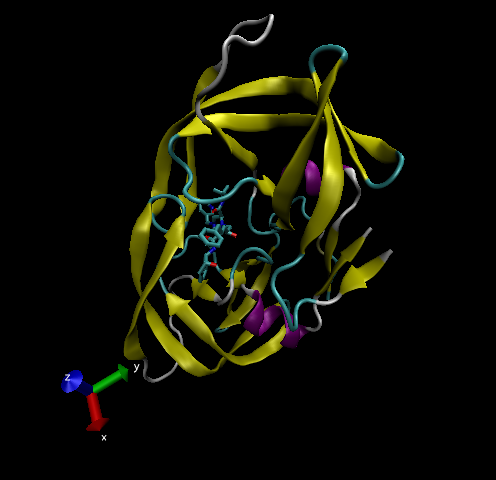
\includegraphics{vmdscene.png}
\caption{VMD rendered image of 1HSG}
\end{figure}

Discussion Topic: Can you think of a way in which indinavir, or even
larger ligands and substrates, could enter the binding site?

\hypertarget{intro-to-bio3d-in-r}{%
\section{Intro to Bio3D in R}\label{intro-to-bio3d-in-r}}

\hypertarget{reading-pdb-file-data-into-r}{%
\subsection{Reading PDB File Data into
R}\label{reading-pdb-file-data-into-r}}

Load the Bio3D package!

\begin{Shaded}
\begin{Highlighting}[]
\CommentTok{\#install.packages("bio3d")}
\FunctionTok{library}\NormalTok{(bio3d)}
\end{Highlighting}
\end{Shaded}

Read a PDB file into R.

\begin{Shaded}
\begin{Highlighting}[]
\NormalTok{hsg }\OtherTok{\textless{}{-}} \FunctionTok{read.pdb}\NormalTok{(}\StringTok{"1hsg"}\NormalTok{)}
\end{Highlighting}
\end{Shaded}

\begin{verbatim}
##   Note: Accessing on-line PDB file
\end{verbatim}

\begin{Shaded}
\begin{Highlighting}[]
\NormalTok{hsg}
\end{Highlighting}
\end{Shaded}

\begin{verbatim}
## 
##  Call:  read.pdb(file = "1hsg")
## 
##    Total Models#: 1
##      Total Atoms#: 1686,  XYZs#: 5058  Chains#: 2  (values: A B)
## 
##      Protein Atoms#: 1514  (residues/Calpha atoms#: 198)
##      Nucleic acid Atoms#: 0  (residues/phosphate atoms#: 0)
## 
##      Non-protein/nucleic Atoms#: 172  (residues: 128)
##      Non-protein/nucleic resid values: [ HOH (127), MK1 (1) ]
## 
##    Protein sequence:
##       PQITLWQRPLVTIKIGGQLKEALLDTGADDTVLEEMSLPGRWKPKMIGGIGGFIKVRQYD
##       QILIEICGHKAIGTVLVGPTPVNIIGRNLLTQIGCTLNFPQITLWQRPLVTIKIGGQLKE
##       ALLDTGADDTVLEEMSLPGRWKPKMIGGIGGFIKVRQYDQILIEICGHKAIGTVLVGPTP
##       VNIIGRNLLTQIGCTLNF
## 
## + attr: atom, xyz, seqres, helix, sheet,
##         calpha, remark, call
\end{verbatim}

\textbf{Q7: How many amino acid residues are there in this pdb object?}

There are 198 amino acid residues in this object.

\textbf{Q8: Name one of the two non-protein residues?}

One of the non-protein residues is HOH, known as water.

\textbf{Q9: How many protein chains are in this structure?}

There are 2 protein chains.

Examine some of the attributes of the PDB object.

\begin{Shaded}
\begin{Highlighting}[]
\FunctionTok{attributes}\NormalTok{(hsg)}
\end{Highlighting}
\end{Shaded}

\begin{verbatim}
## $names
## [1] "atom"   "xyz"    "seqres" "helix"  "sheet"  "calpha" "remark" "call"  
## 
## $class
## [1] "pdb" "sse"
\end{verbatim}

\begin{Shaded}
\begin{Highlighting}[]
\FunctionTok{head}\NormalTok{(hsg}\SpecialCharTok{$}\NormalTok{atom)}
\end{Highlighting}
\end{Shaded}

\begin{verbatim}
##   type eleno elety  alt resid chain resno insert      x      y     z o     b
## 1 ATOM     1     N <NA>   PRO     A     1   <NA> 29.361 39.686 5.862 1 38.10
## 2 ATOM     2    CA <NA>   PRO     A     1   <NA> 30.307 38.663 5.319 1 40.62
## 3 ATOM     3     C <NA>   PRO     A     1   <NA> 29.760 38.071 4.022 1 42.64
## 4 ATOM     4     O <NA>   PRO     A     1   <NA> 28.600 38.302 3.676 1 43.40
## 5 ATOM     5    CB <NA>   PRO     A     1   <NA> 30.508 37.541 6.342 1 37.87
## 6 ATOM     6    CG <NA>   PRO     A     1   <NA> 29.296 37.591 7.162 1 38.40
##   segid elesy charge
## 1  <NA>     N   <NA>
## 2  <NA>     C   <NA>
## 3  <NA>     C   <NA>
## 4  <NA>     O   <NA>
## 5  <NA>     C   <NA>
## 6  <NA>     C   <NA>
\end{verbatim}

\hypertarget{comparative-structure-analysis-of-adenylate-kinase}{%
\section{Comparative Structure Analysis of Adenylate
Kinase}\label{comparative-structure-analysis-of-adenylate-kinase}}

\hypertarget{set-up}{%
\subsection{Set-up}\label{set-up}}

Install the following in the R console.

\begin{Shaded}
\begin{Highlighting}[]
\CommentTok{\#install.packages("ggrepel")}
\CommentTok{\#install.packages("devtools")}
\CommentTok{\#install.packages("BiocManager")}

\CommentTok{\#BiocManager::install("msa")}
\CommentTok{\#devtools::install\_bitbucket("Grantlab/bio3d{-}view")}
\end{Highlighting}
\end{Shaded}

\textbf{Q10. Which of the packages above is found only on BioConductor
and not CRAN?}

The ``msa'' package is found only on BioConductor.

\textbf{Q11. Which of the above packages is not found on BioConductor or
CRAN?}

The ``bio3d-view'' package isn't found on either BioConductor or CRAN.

\textbf{Q12. True or False? Functions from the devtools package can be
used to install packages from GitHub and BitBucket?}

TRUE.

\hypertarget{search-retrieve-adk-structures}{%
\subsection{Search \& Retrieve ADK
Structures}\label{search-retrieve-adk-structures}}

First, we need to find the sequence of chain A of 1AKE.

\begin{Shaded}
\begin{Highlighting}[]
\NormalTok{aa }\OtherTok{\textless{}{-}} \FunctionTok{get.seq}\NormalTok{(}\StringTok{"1ake\_A"}\NormalTok{)}
\end{Highlighting}
\end{Shaded}

\begin{verbatim}
## Warning in get.seq("1ake_A"): Removing existing file: seqs.fasta
\end{verbatim}

\begin{verbatim}
## Fetching... Please wait. Done.
\end{verbatim}

\begin{Shaded}
\begin{Highlighting}[]
\NormalTok{aa}
\end{Highlighting}
\end{Shaded}

\begin{verbatim}
##              1        .         .         .         .         .         60 
## pdb|1AKE|A   MRIILLGAPGAGKGTQAQFIMEKYGIPQISTGDMLRAAVKSGSELGKQAKDIMDAGKLVT
##              1        .         .         .         .         .         60 
## 
##             61        .         .         .         .         .         120 
## pdb|1AKE|A   DELVIALVKERIAQEDCRNGFLLDGFPRTIPQADAMKEAGINVDYVLEFDVPDELIVDRI
##             61        .         .         .         .         .         120 
## 
##            121        .         .         .         .         .         180 
## pdb|1AKE|A   VGRRVHAPSGRVYHVKFNPPKVEGKDDVTGEELTTRKDDQEETVRKRLVEYHQMTAPLIG
##            121        .         .         .         .         .         180 
## 
##            181        .         .         .   214 
## pdb|1AKE|A   YYSKEAEAGNTKYAKVDGTKPVAEVRADLEKILG
##            181        .         .         .   214 
## 
## Call:
##   read.fasta(file = outfile)
## 
## Class:
##   fasta
## 
## Alignment dimensions:
##   1 sequence rows; 214 position columns (214 non-gap, 0 gap) 
## 
## + attr: id, ali, call
\end{verbatim}

\textbf{Q13. How many amino acids are in this sequence, i.e.~how long is
this sequence?}

There are 214 amino acids in the sequence.

Now we can use this sequence to BLAST search the PDB database to find
similar sequences.

\begin{Shaded}
\begin{Highlighting}[]
\NormalTok{aa\_blast }\OtherTok{\textless{}{-}} \FunctionTok{blast.pdb}\NormalTok{(aa)}
\end{Highlighting}
\end{Shaded}

\begin{verbatim}
##  Searching ... please wait (updates every 5 seconds) RID = 11C2JHTB013 
##  ......................
##  Reporting 100 hits
\end{verbatim}

We can visualize and filter the BLAST results using the function
plot.blast().

\begin{Shaded}
\begin{Highlighting}[]
\NormalTok{hits }\OtherTok{\textless{}{-}} \FunctionTok{plot.blast}\NormalTok{(aa\_blast)}
\end{Highlighting}
\end{Shaded}

\begin{verbatim}
##   * Possible cutoff values:    197 -3 
##             Yielding Nhits:    16 100 
## 
##   * Chosen cutoff value of:    197 
##             Yielding Nhits:    16
\end{verbatim}

\includegraphics{class09_files/figure-latex/unnamed-chunk-12-1.pdf}

Here, we can see the top scoring hits from the BLAST results.

\begin{Shaded}
\begin{Highlighting}[]
\FunctionTok{head}\NormalTok{(hits}\SpecialCharTok{$}\NormalTok{pdb.id)}
\end{Highlighting}
\end{Shaded}

\begin{verbatim}
## [1] "1AKE_A" "4X8M_A" "6S36_A" "6RZE_A" "4X8H_A" "3HPR_A"
\end{verbatim}

With the above information, we can use get.pdb() to fetch and parse the
dientified structures.

\begin{Shaded}
\begin{Highlighting}[]
\CommentTok{\# Download releated PDB files}
\NormalTok{files }\OtherTok{\textless{}{-}} \FunctionTok{get.pdb}\NormalTok{(hits}\SpecialCharTok{$}\NormalTok{pdb.id, }\AttributeTok{path =} \StringTok{"pdbs"}\NormalTok{, }\AttributeTok{split =} \ConstantTok{TRUE}\NormalTok{, }\AttributeTok{gzip =} \ConstantTok{TRUE}\NormalTok{)}
\end{Highlighting}
\end{Shaded}

\begin{verbatim}
## Warning in get.pdb(hits$pdb.id, path = "pdbs", split = TRUE, gzip = TRUE): pdbs/
## 1AKE.pdb exists. Skipping download
\end{verbatim}

\begin{verbatim}
## Warning in get.pdb(hits$pdb.id, path = "pdbs", split = TRUE, gzip = TRUE): pdbs/
## 4X8M.pdb exists. Skipping download
\end{verbatim}

\begin{verbatim}
## Warning in get.pdb(hits$pdb.id, path = "pdbs", split = TRUE, gzip = TRUE): pdbs/
## 6S36.pdb exists. Skipping download
\end{verbatim}

\begin{verbatim}
## Warning in get.pdb(hits$pdb.id, path = "pdbs", split = TRUE, gzip = TRUE): pdbs/
## 6RZE.pdb exists. Skipping download
\end{verbatim}

\begin{verbatim}
## Warning in get.pdb(hits$pdb.id, path = "pdbs", split = TRUE, gzip = TRUE): pdbs/
## 4X8H.pdb exists. Skipping download
\end{verbatim}

\begin{verbatim}
## Warning in get.pdb(hits$pdb.id, path = "pdbs", split = TRUE, gzip = TRUE): pdbs/
## 3HPR.pdb exists. Skipping download
\end{verbatim}

\begin{verbatim}
## Warning in get.pdb(hits$pdb.id, path = "pdbs", split = TRUE, gzip = TRUE): pdbs/
## 1E4V.pdb exists. Skipping download
\end{verbatim}

\begin{verbatim}
## Warning in get.pdb(hits$pdb.id, path = "pdbs", split = TRUE, gzip = TRUE): pdbs/
## 5EJE.pdb exists. Skipping download
\end{verbatim}

\begin{verbatim}
## Warning in get.pdb(hits$pdb.id, path = "pdbs", split = TRUE, gzip = TRUE): pdbs/
## 1E4Y.pdb exists. Skipping download
\end{verbatim}

\begin{verbatim}
## Warning in get.pdb(hits$pdb.id, path = "pdbs", split = TRUE, gzip = TRUE): pdbs/
## 3X2S.pdb exists. Skipping download
\end{verbatim}

\begin{verbatim}
## Warning in get.pdb(hits$pdb.id, path = "pdbs", split = TRUE, gzip = TRUE): pdbs/
## 6HAP.pdb exists. Skipping download
\end{verbatim}

\begin{verbatim}
## Warning in get.pdb(hits$pdb.id, path = "pdbs", split = TRUE, gzip = TRUE): pdbs/
## 6HAM.pdb exists. Skipping download
\end{verbatim}

\begin{verbatim}
## Warning in get.pdb(hits$pdb.id, path = "pdbs", split = TRUE, gzip = TRUE): pdbs/
## 4K46.pdb exists. Skipping download
\end{verbatim}

\begin{verbatim}
## Warning in get.pdb(hits$pdb.id, path = "pdbs", split = TRUE, gzip = TRUE): pdbs/
## 4NP6.pdb exists. Skipping download
\end{verbatim}

\begin{verbatim}
## Warning in get.pdb(hits$pdb.id, path = "pdbs", split = TRUE, gzip = TRUE): pdbs/
## 3GMT.pdb exists. Skipping download
\end{verbatim}

\begin{verbatim}
## Warning in get.pdb(hits$pdb.id, path = "pdbs", split = TRUE, gzip = TRUE): pdbs/
## 4PZL.pdb exists. Skipping download
\end{verbatim}

\begin{verbatim}
##   |                                                                              |                                                                      |   0%  |                                                                              |====                                                                  |   6%  |                                                                              |=========                                                             |  12%  |                                                                              |=============                                                         |  19%  |                                                                              |==================                                                    |  25%  |                                                                              |======================                                                |  31%  |                                                                              |==========================                                            |  38%  |                                                                              |===============================                                       |  44%  |                                                                              |===================================                                   |  50%  |                                                                              |=======================================                               |  56%  |                                                                              |============================================                          |  62%  |                                                                              |================================================                      |  69%  |                                                                              |====================================================                  |  75%  |                                                                              |=========================================================             |  81%  |                                                                              |=============================================================         |  88%  |                                                                              |==================================================================    |  94%  |                                                                              |======================================================================| 100%
\end{verbatim}

\hypertarget{align-and-superpose-structures}{%
\subsection{Align and Superpose
Structures}\label{align-and-superpose-structures}}

The code below will align and fit the identified PDB structures.

\begin{Shaded}
\begin{Highlighting}[]
\CommentTok{\#align PDBs}
\NormalTok{pdbs }\OtherTok{\textless{}{-}} \FunctionTok{pdbaln}\NormalTok{(files, }\AttributeTok{fit =} \ConstantTok{TRUE}\NormalTok{, }\AttributeTok{exefile =} \StringTok{"msa"}\NormalTok{)}
\end{Highlighting}
\end{Shaded}

\begin{verbatim}
## Reading PDB files:
## pdbs/split_chain/1AKE_A.pdb
## pdbs/split_chain/4X8M_A.pdb
## pdbs/split_chain/6S36_A.pdb
## pdbs/split_chain/6RZE_A.pdb
## pdbs/split_chain/4X8H_A.pdb
## pdbs/split_chain/3HPR_A.pdb
## pdbs/split_chain/1E4V_A.pdb
## pdbs/split_chain/5EJE_A.pdb
## pdbs/split_chain/1E4Y_A.pdb
## pdbs/split_chain/3X2S_A.pdb
## pdbs/split_chain/6HAP_A.pdb
## pdbs/split_chain/6HAM_A.pdb
## pdbs/split_chain/4K46_A.pdb
## pdbs/split_chain/4NP6_A.pdb
## pdbs/split_chain/3GMT_A.pdb
## pdbs/split_chain/4PZL_A.pdb
##    PDB has ALT records, taking A only, rm.alt=TRUE
## ..   PDB has ALT records, taking A only, rm.alt=TRUE
## .   PDB has ALT records, taking A only, rm.alt=TRUE
## ..   PDB has ALT records, taking A only, rm.alt=TRUE
## ..   PDB has ALT records, taking A only, rm.alt=TRUE
## ....   PDB has ALT records, taking A only, rm.alt=TRUE
## .   PDB has ALT records, taking A only, rm.alt=TRUE
## ....
## 
## Extracting sequences
## 
## pdb/seq: 1   name: pdbs/split_chain/1AKE_A.pdb 
##    PDB has ALT records, taking A only, rm.alt=TRUE
## pdb/seq: 2   name: pdbs/split_chain/4X8M_A.pdb 
## pdb/seq: 3   name: pdbs/split_chain/6S36_A.pdb 
##    PDB has ALT records, taking A only, rm.alt=TRUE
## pdb/seq: 4   name: pdbs/split_chain/6RZE_A.pdb 
##    PDB has ALT records, taking A only, rm.alt=TRUE
## pdb/seq: 5   name: pdbs/split_chain/4X8H_A.pdb 
## pdb/seq: 6   name: pdbs/split_chain/3HPR_A.pdb 
##    PDB has ALT records, taking A only, rm.alt=TRUE
## pdb/seq: 7   name: pdbs/split_chain/1E4V_A.pdb 
## pdb/seq: 8   name: pdbs/split_chain/5EJE_A.pdb 
##    PDB has ALT records, taking A only, rm.alt=TRUE
## pdb/seq: 9   name: pdbs/split_chain/1E4Y_A.pdb 
## pdb/seq: 10   name: pdbs/split_chain/3X2S_A.pdb 
## pdb/seq: 11   name: pdbs/split_chain/6HAP_A.pdb 
## pdb/seq: 12   name: pdbs/split_chain/6HAM_A.pdb 
##    PDB has ALT records, taking A only, rm.alt=TRUE
## pdb/seq: 13   name: pdbs/split_chain/4K46_A.pdb 
##    PDB has ALT records, taking A only, rm.alt=TRUE
## pdb/seq: 14   name: pdbs/split_chain/4NP6_A.pdb 
## pdb/seq: 15   name: pdbs/split_chain/3GMT_A.pdb 
## pdb/seq: 16   name: pdbs/split_chain/4PZL_A.pdb
\end{verbatim}

\begin{Shaded}
\begin{Highlighting}[]
\CommentTok{\#vector containing PDB codes for figure axis}
\NormalTok{ids }\OtherTok{\textless{}{-}} \FunctionTok{basename.pdb}\NormalTok{(pdbs}\SpecialCharTok{$}\NormalTok{id)}

\CommentTok{\#draw schematic alignment}
\FunctionTok{plot}\NormalTok{(pdbs, }\AttributeTok{labels =}\NormalTok{ ids)}
\end{Highlighting}
\end{Shaded}

\includegraphics{class09_files/figure-latex/unnamed-chunk-15-1.pdf}

\hypertarget{viewing-the-superposed-structures-optional}{%
\subsection{Viewing the Superposed Structures
{[}OPTIONAL{]}}\label{viewing-the-superposed-structures-optional}}

\begin{Shaded}
\begin{Highlighting}[]
\CommentTok{\#install.packages("devtools")}
\CommentTok{\#library(devtools)}
\CommentTok{\#install\_bitbucket("Grantlab/bio3d{-}view")}
\CommentTok{\#install.packages("rgl")}

\FunctionTok{library}\NormalTok{(bio3d.view)}
\FunctionTok{library}\NormalTok{(rgl)}

\FunctionTok{view.pdbs}\NormalTok{(pdbs)}
\end{Highlighting}
\end{Shaded}

{[}viewer works! :){]}

\hypertarget{annotate-pdb-structures}{%
\subsection{Annotate PDB Structures}\label{annotate-pdb-structures}}

The functions below help us annotate the PDB structures so we can
associate each structure with its source species.

\begin{Shaded}
\begin{Highlighting}[]
\NormalTok{anno }\OtherTok{\textless{}{-}} \FunctionTok{pdb.annotate}\NormalTok{(}\FunctionTok{c}\NormalTok{(}\StringTok{"2mh3\_A"}\NormalTok{, }\StringTok{"4f3l"}\NormalTok{), }\AttributeTok{anno.terms =} \FunctionTok{c}\NormalTok{(}\StringTok{"structureId"}\NormalTok{, }\StringTok{"experimentalTechnique"}\NormalTok{, }\StringTok{"resolution"}\NormalTok{,}\StringTok{"pfam"}\NormalTok{, }\StringTok{"source"}\NormalTok{, }\StringTok{"citation"}\NormalTok{))}
\NormalTok{anno}
\end{Highlighting}
\end{Shaded}

\begin{verbatim}
##        structureId experimentalTechnique resolution
## 2MH3_A        2MH3                   NMR         NA
## 4F3L_B        4F3L                 X-ray      2.268
## 4F3L_A        4F3L                 X-ray      2.268
##                                             pfam       source
## 2MH3_A Helix-loop-helix DNA-binding domain (HLH) Homo sapiens
## 4F3L_B                       PAS domain (PAS_11) Mus musculus
## 4F3L_A                       PAS domain (PAS_11) Mus musculus
##                                   citation
## 2MH3_A Popovic, M., et al. Proteins (2014)
## 4F3L_B    Huang, N., et al. Science (2012)
## 4F3L_A    Huang, N., et al. Science (2012)
\end{verbatim}

\hypertarget{principal-component-analysis}{%
\subsection{Principal Component
Analysis}\label{principal-component-analysis}}

We can use PCA on the identified PDBs in order to determine any
significant structural variations.

\begin{Shaded}
\begin{Highlighting}[]
\NormalTok{pc.xray }\OtherTok{\textless{}{-}} \FunctionTok{pca}\NormalTok{(pdbs)}
\FunctionTok{plot}\NormalTok{(pc.xray)}
\end{Highlighting}
\end{Shaded}

\includegraphics{class09_files/figure-latex/unnamed-chunk-18-1.pdf}

We can calculate the pairwise RMSD values of the structures, which can
help with clutering analysis.

\begin{Shaded}
\begin{Highlighting}[]
\CommentTok{\#calculate RMSD}
\NormalTok{rd }\OtherTok{\textless{}{-}} \FunctionTok{rmsd}\NormalTok{(pdbs)}
\end{Highlighting}
\end{Shaded}

\begin{verbatim}
## Warning in rmsd(pdbs): No indices provided, using the 204 non NA positions
\end{verbatim}

\begin{Shaded}
\begin{Highlighting}[]
\CommentTok{\#structure{-}based clustering}
\NormalTok{hc.rd }\OtherTok{\textless{}{-}} \FunctionTok{hclust}\NormalTok{(}\FunctionTok{dist}\NormalTok{(rd))}
\NormalTok{grps.rd }\OtherTok{\textless{}{-}} \FunctionTok{cutree}\NormalTok{(hc.rd, }\AttributeTok{k =} \DecValTok{3}\NormalTok{)}

\FunctionTok{plot}\NormalTok{(pc.xray, }\DecValTok{1}\SpecialCharTok{:}\DecValTok{2}\NormalTok{, }\AttributeTok{col=}\StringTok{"grey50"}\NormalTok{, }\AttributeTok{bg =}\NormalTok{ grps.rd, }\AttributeTok{pch =} \DecValTok{21}\NormalTok{, }\AttributeTok{cex =} \DecValTok{1}\NormalTok{)}
\end{Highlighting}
\end{Shaded}

\includegraphics{class09_files/figure-latex/unnamed-chunk-19-1.pdf}

\hypertarget{normal-mode-analysis-optional}{%
\section{Normal Mode Analysis
{[}OPTIONAL{]}}\label{normal-mode-analysis-optional}}

Normal Mode Analysis on PDBs can help with characterizing the profiles
of related protein structures.

\begin{Shaded}
\begin{Highlighting}[]
\NormalTok{modes }\OtherTok{\textless{}{-}} \FunctionTok{nma}\NormalTok{(pdbs)}
\end{Highlighting}
\end{Shaded}

\begin{verbatim}
## 
## Details of Scheduled Calculation:
##   ... 16 input structures 
##   ... storing 606 eigenvectors for each structure 
##   ... dimension of x$U.subspace: ( 612x606x16 )
##   ... coordinate superposition prior to NM calculation 
##   ... aligned eigenvectors (gap containing positions removed)  
##   ... estimated memory usage of final 'eNMA' object: 45.4 Mb 
## 
##   |                                                                              |                                                                      |   0%  |                                                                              |====                                                                  |   6%  |                                                                              |=========                                                             |  12%  |                                                                              |=============                                                         |  19%  |                                                                              |==================                                                    |  25%  |                                                                              |======================                                                |  31%  |                                                                              |==========================                                            |  38%  |                                                                              |===============================                                       |  44%  |                                                                              |===================================                                   |  50%  |                                                                              |=======================================                               |  56%  |                                                                              |============================================                          |  62%  |                                                                              |================================================                      |  69%  |                                                                              |====================================================                  |  75%  |                                                                              |=========================================================             |  81%  |                                                                              |=============================================================         |  88%  |                                                                              |==================================================================    |  94%  |                                                                              |======================================================================| 100%
\end{verbatim}

\begin{Shaded}
\begin{Highlighting}[]
\FunctionTok{plot}\NormalTok{(modes, pdbs, }\AttributeTok{col =}\NormalTok{ grps.rd)}
\end{Highlighting}
\end{Shaded}

\begin{verbatim}
## Extracting SSE from pdbs$sse attribute
\end{verbatim}

\includegraphics{class09_files/figure-latex/unnamed-chunk-20-1.pdf}

\textbf{Q14. What do you note about this plot? Are the black and colored
lines similar or different? Where do you think they differ most and
why?}

The black lines and colored lines differ at certain regions,
particularly from around residue numbers 30-70 and residue numbers
125-175. These differences may be due to those residues being associated
with ligand binding sites for the structures represented by the colored
lines.

\end{document}
